\documentclass[12pt, a4paper]{report}
\usepackage[top=1cm, left=1cm, right=1cm]{geometry}

\usepackage[utf8]{inputenc}
\usepackage[russian]{babel}

\usepackage{array}
\newcolumntype{M}[1]{>{\centering\arraybackslash}m{#1}}

\usepackage{hyperref}
\hypersetup{
	colorlinks,
	citecolor=black,
	filecolor=black,
	linkcolor=black,
	urlcolor=black
}

\usepackage{sectsty}
\allsectionsfont{\centering}

\usepackage{indentfirst}
\setlength\parindent{24pt}

\usepackage{makecell}

\usepackage{amsmath}

\def\H{\rule{0pt}{1.5ex}H}

\usepackage{graphicx}
\graphicspath{ {assets/initial/} {assets/results/} }
\usepackage[export]{adjustbox}

\begin{document}
	\begin{titlepage}
		\begin{center}
			\large \textbf{Министерство науки и высшего образования Российской Федерации} \\
			\large \textbf{Федеральное государственное бюджетное образовательное учреждение высшего образования} \\
			\large \textbf{«Российский химико-технологический университет имени Д.И. Менделеева»} \\

			\vspace*{4cm}
			\LARGE \textbf{ОТЧЕТ ПО ЛАБОРАТОРНОЙ РАБОТЕ} \\
			\Large \textbf{Серментация частиц}

			\vspace*{4cm}
			\begin{flushright}
				\Large
				\begin{tabular}{>{\raggedleft\arraybackslash}p{9cm} p{10cm}}
					Выполнил студент группы КС-36: & Золотухин Андрей Александрович \\
					Ссылка на репозиторий: & https://github.com/ \\
					& CorgiPuppy/ \\
					& big-data-labs \\
					Принял: & Зубов Дмитрий Владимирович \\
					Дата сдачи: & 05.06.2025 \\
				\end{tabular}
			\end{flushright}

			\vspace*{5cm}
			\Large \textbf{Москва \\ 2025}
		\end{center}
	\end{titlepage}

	\tableofcontents
	\thispagestyle{empty}
	\newpage

	\pagenumbering{arabic}

	\section*{Описание задачи}
	\addcontentsline{toc}{section}{Описание задачи}
	\large

	\subsection*{Исходные данные}
	\addcontentsline{toc}{subsection}{Исходные данные}
	\large
	\begin{figure}[h]
		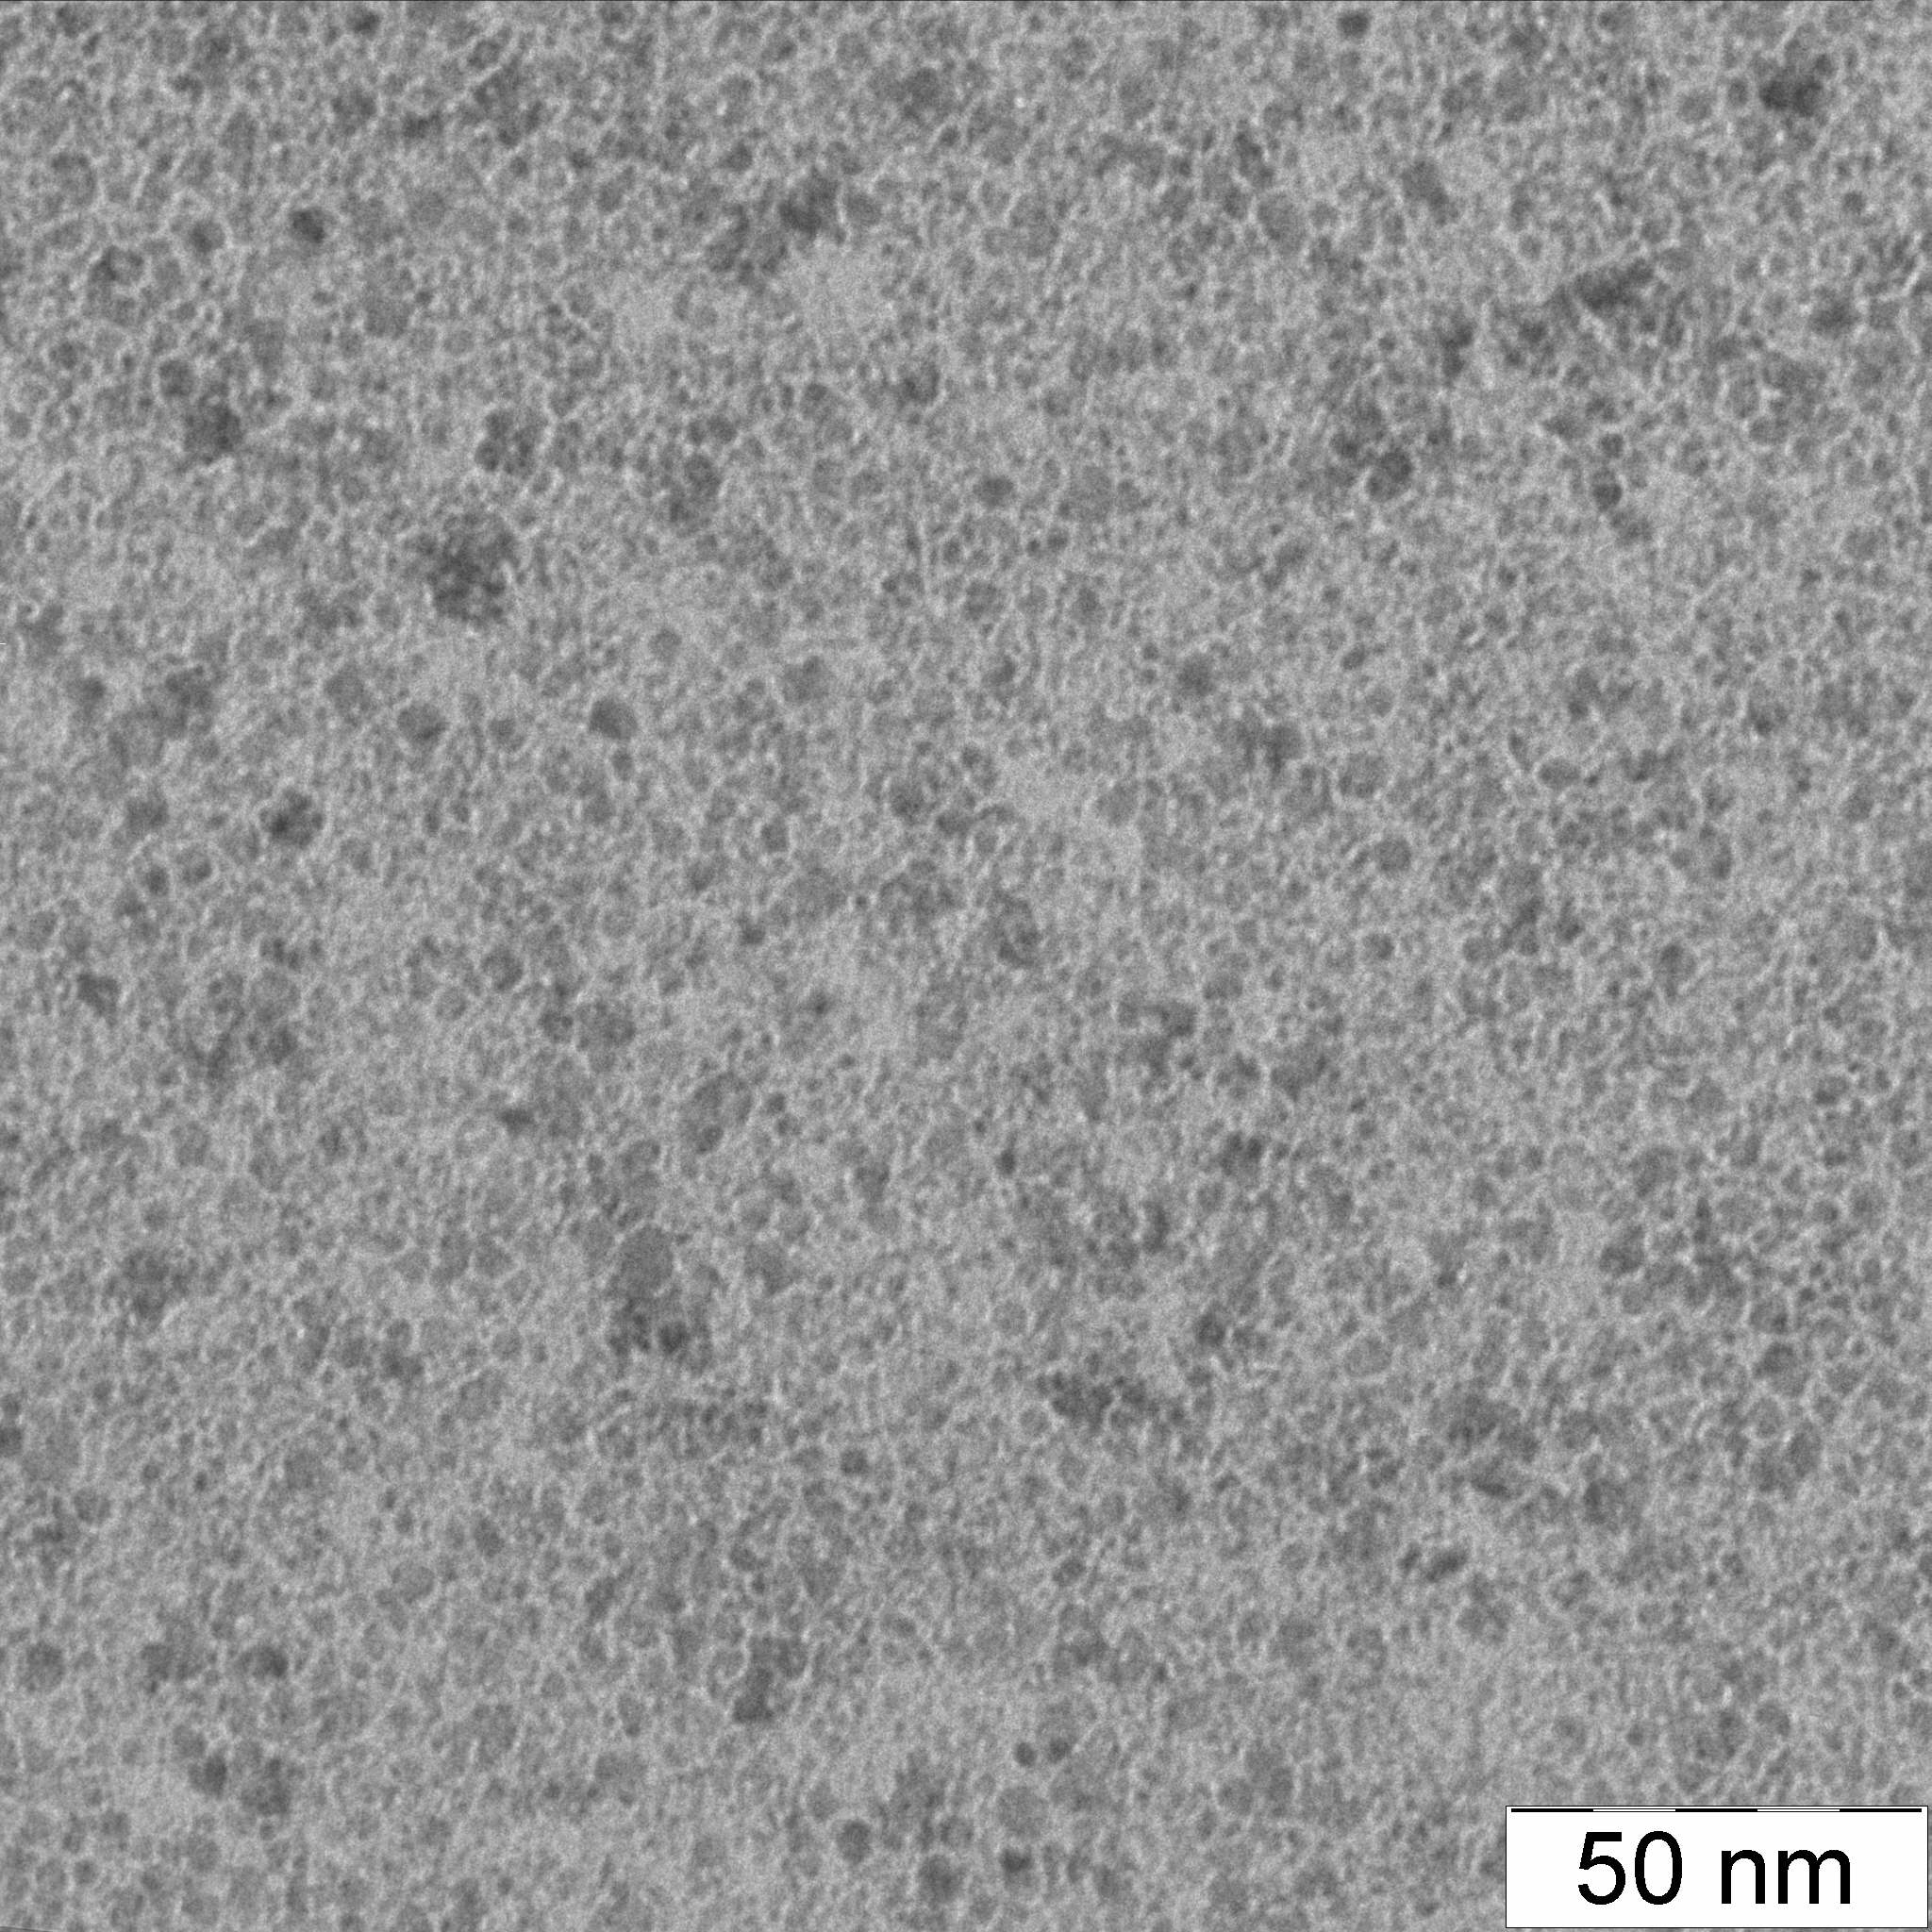
\includegraphics[width=300pt,center]{Image5.jpg}
		\caption{Снимок 5}
	\end{figure}
	\begin{figure}[h]
		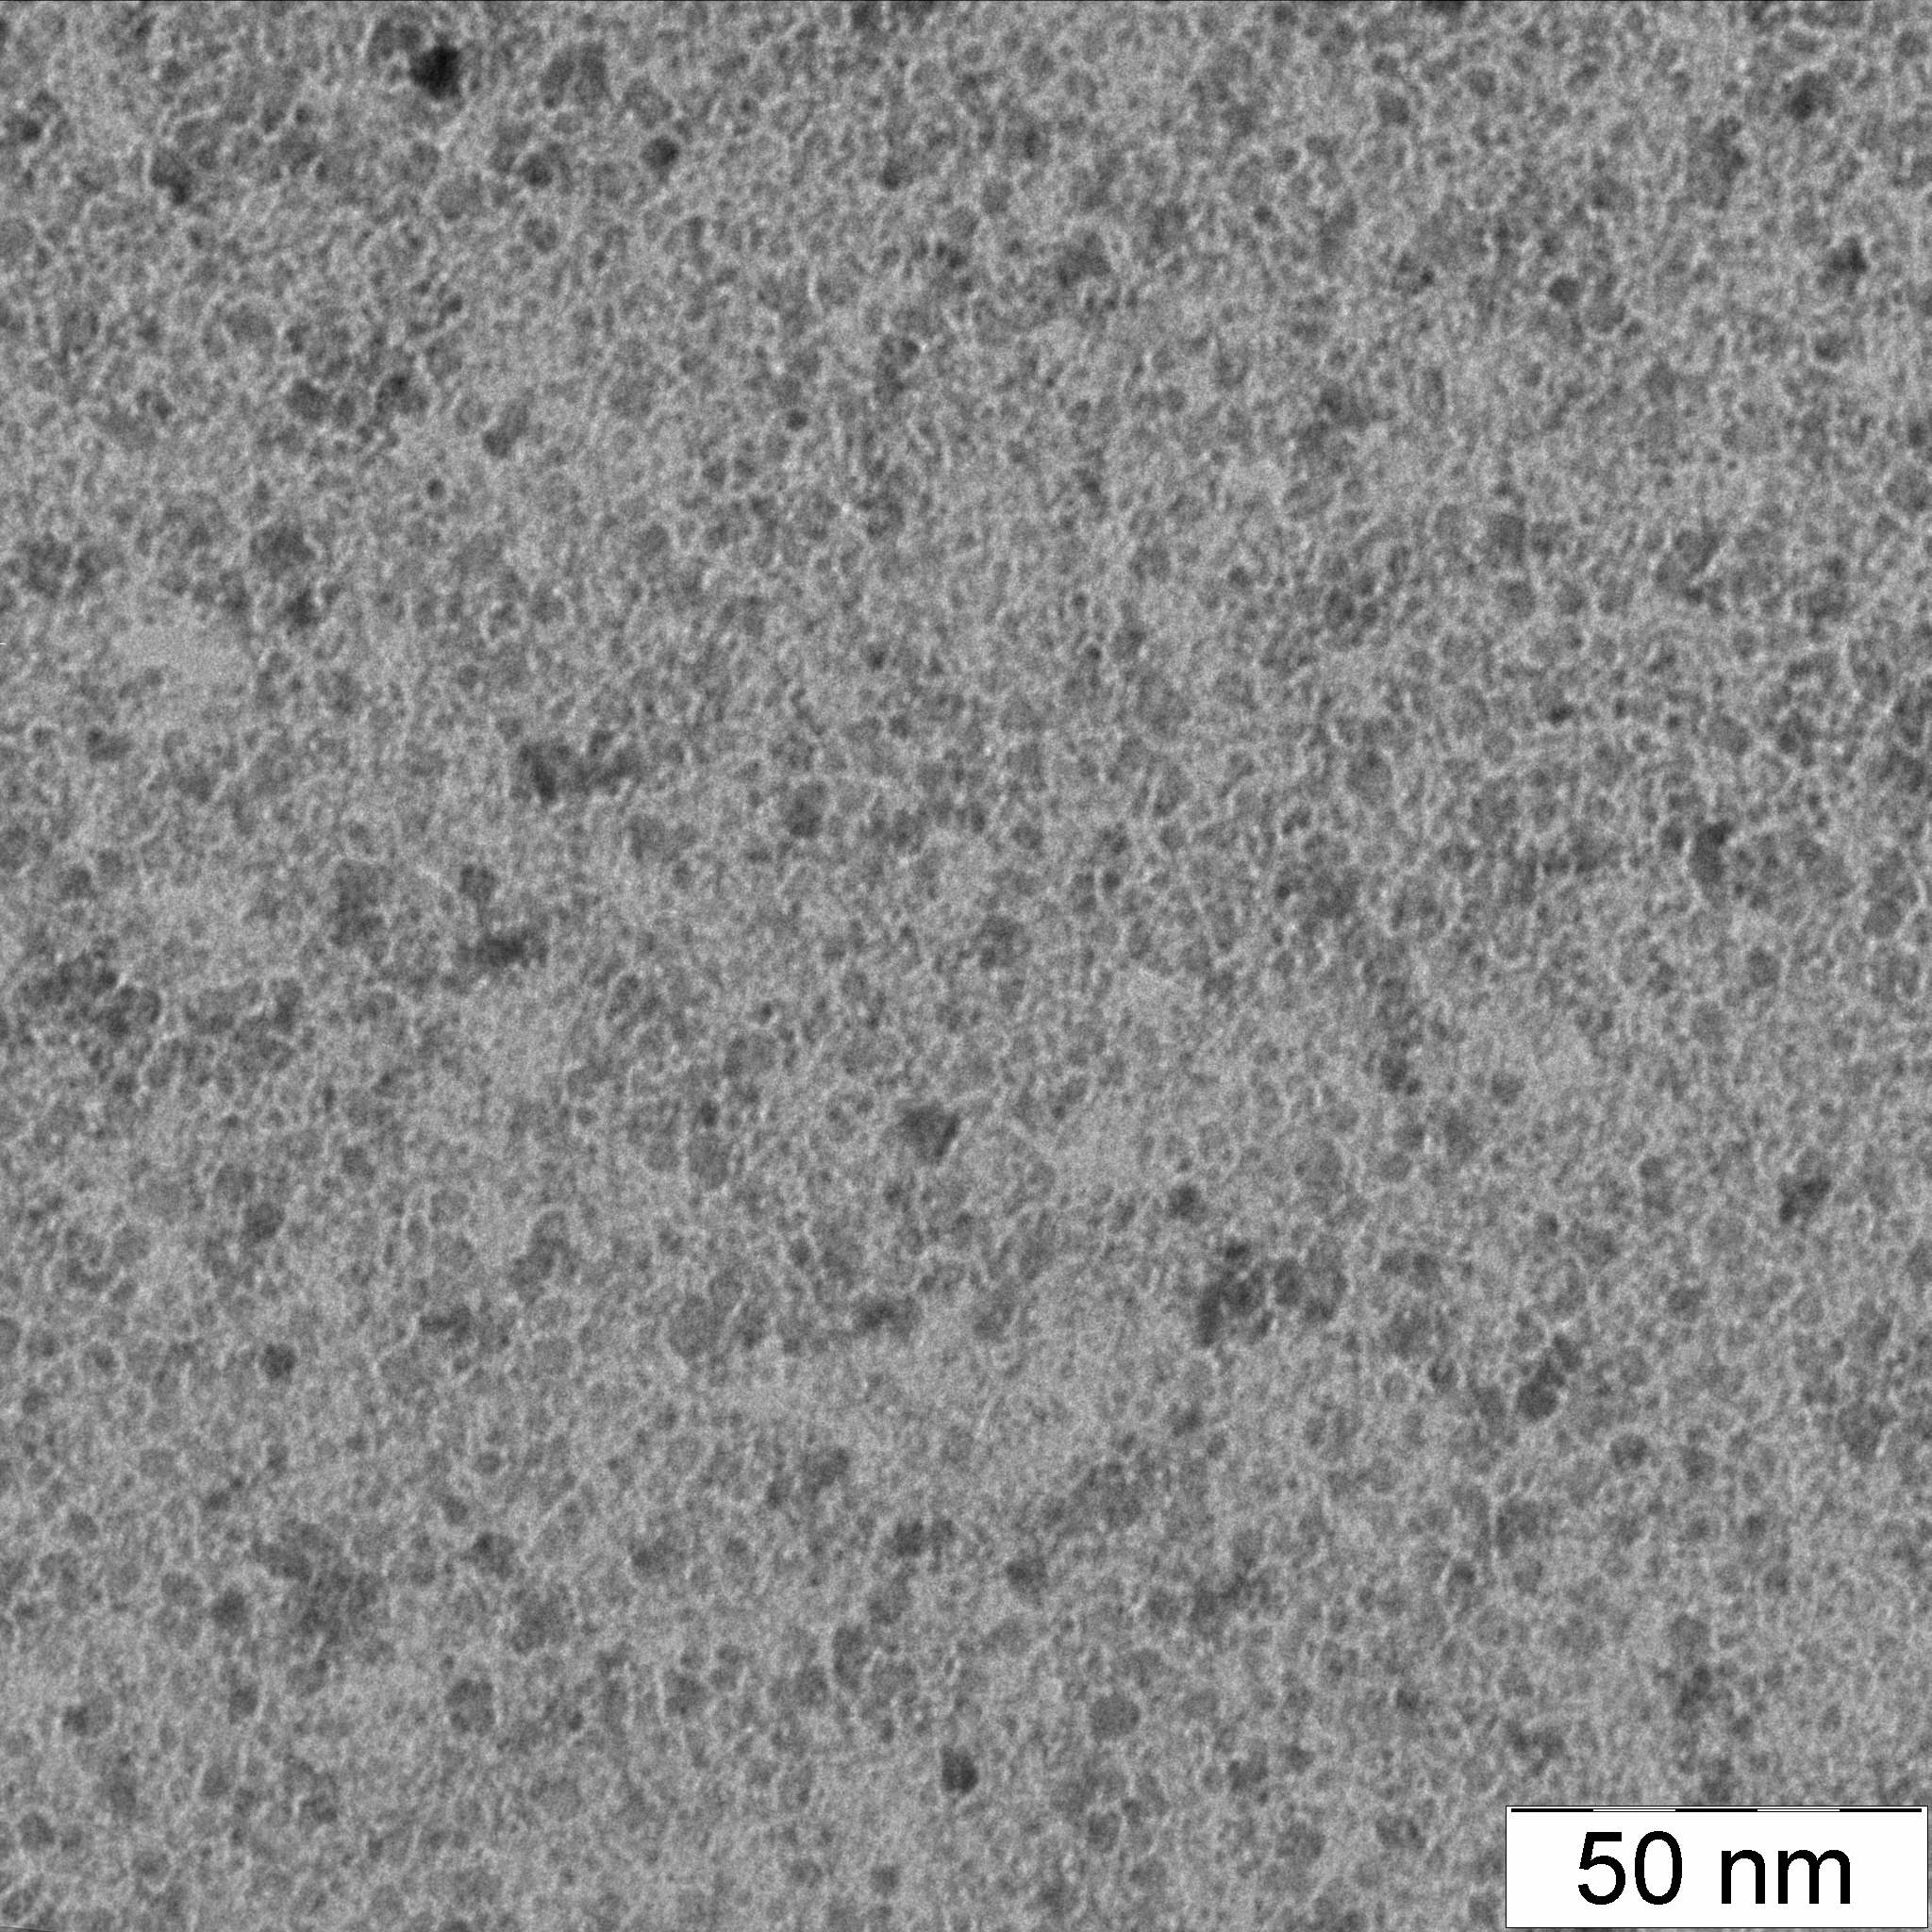
\includegraphics[width=300pt,center]{Image6.jpg}
		\caption{Снимок 6}
	\end{figure}

	\newpage

	\section*{Описание метода/модели}
	\addcontentsline{toc}{section}{Описание метода/модели}
	\large

	\newpage

	\section*{Выполнение задачи}
	\addcontentsline{toc}{section}{Выполнение задачи}

	\newpage
	\vfill

	\subsection*{Подготовительные данные}
	\addcontentsline{toc}{subsection}{Подготовительные данные}
	\large

	\subsubsection*{Valid Dataset}
	\large
	\begin{figure}[h]
		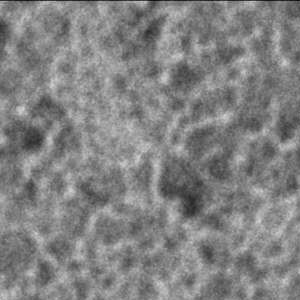
\includegraphics[width=250pt,center]{Image6_300_300.jpg}
		\caption{Вырезанное из снимка 6 изображние 300 на 300 пикселей}
	\end{figure}
	\begin{figure}
		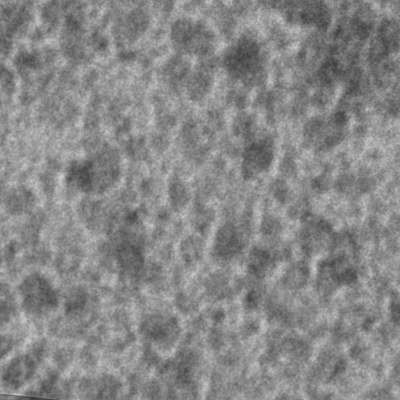
\includegraphics[width=250pt,center]{Image6_400_400.jpg}
		\caption{Вырезанное из снимка 6 изображние 400 на 400 пикселей}
	\end{figure}
	\begin{figure}
		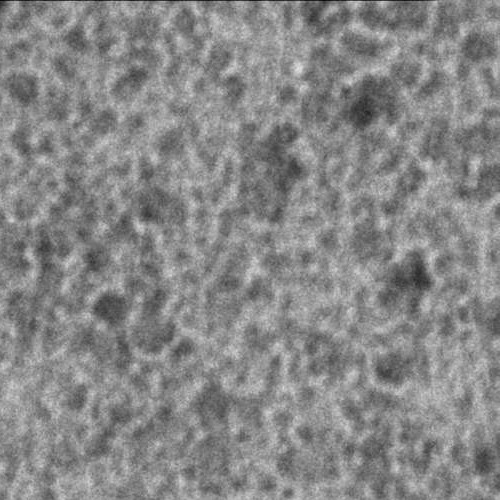
\includegraphics[width=250pt,center]{Image6_500_500.jpg}
		\caption{Вырезанное из снимка 6 изображние 500 на 500 пикселей}
	\end{figure}

	\newpage

	\subsubsection*{Test Dataset}
	\large
	\begin{figure}[h]
		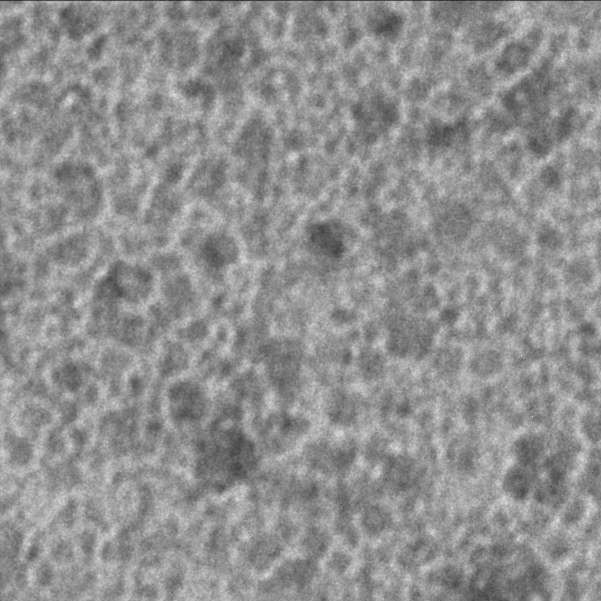
\includegraphics[width=250pt,center]{Image5_601_601.jpg}
		\caption{Вырезанное из снимка 5 изображние 601 на 601 пикселей}
	\end{figure}
	\begin{figure}
		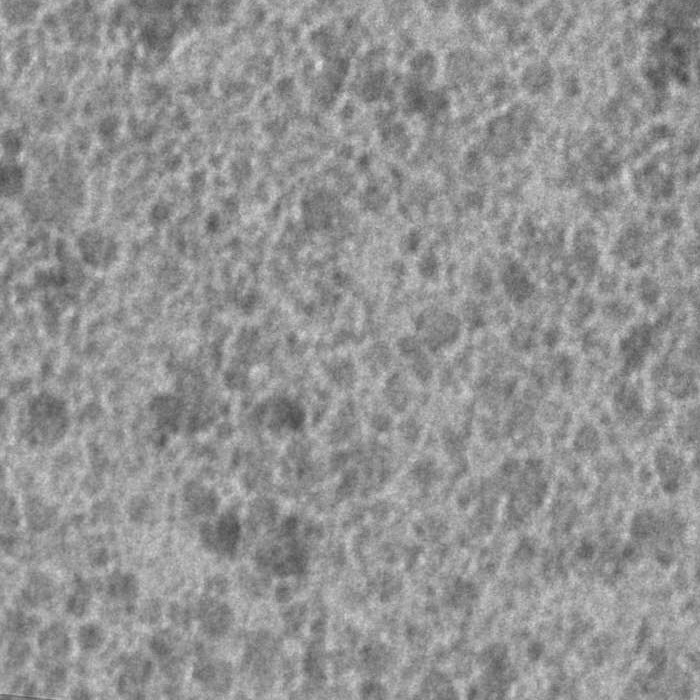
\includegraphics[width=250pt,center]{Image5_700_700.jpg}
		\caption{Вырезанное из снимка 5 изображние 700 на 700 пикселей}
	\end{figure}
	\begin{figure}
		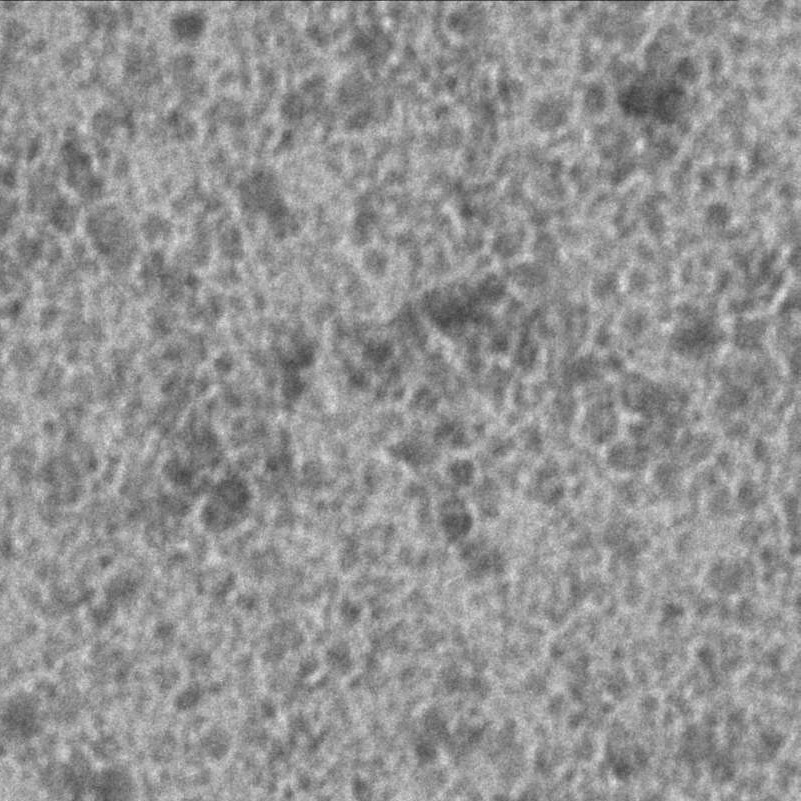
\includegraphics[width=250pt,center]{Image5_801_801.jpg}
		\caption{Вырезанное из снимка 5 изображние 801 на 801 пикселей}
	\end{figure}

	\newpage

	\subsubsection*{Train Dataset}
	\large
	\begin{figure}[h]
		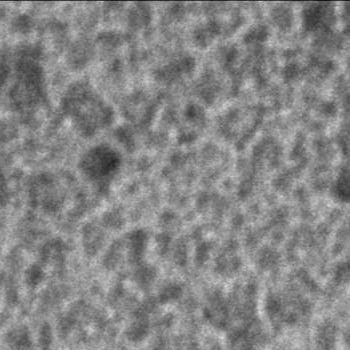
\includegraphics[width=250pt,center]{Image6_350_350.jpg}
		\caption{Вырезанное из снимка 6 изображние 350 на 350 пикселей}
	\end{figure}
	\begin{figure}
		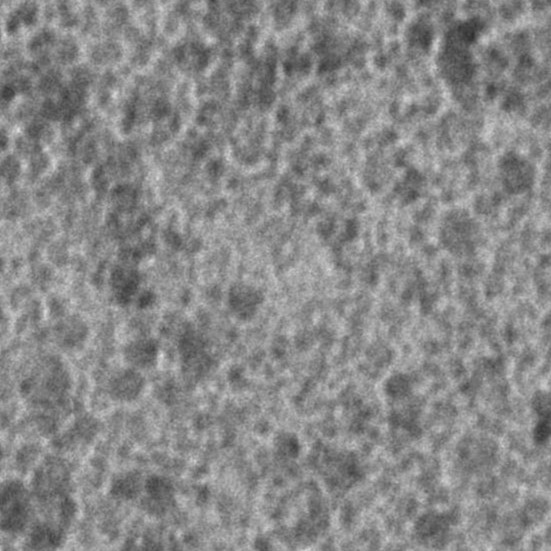
\includegraphics[width=250pt,center]{Image6_551_551.jpg}
		\caption{Вырезанное из снимка 6 изображние 551 на 551 пикселей}
	\end{figure}
	\begin{figure}
		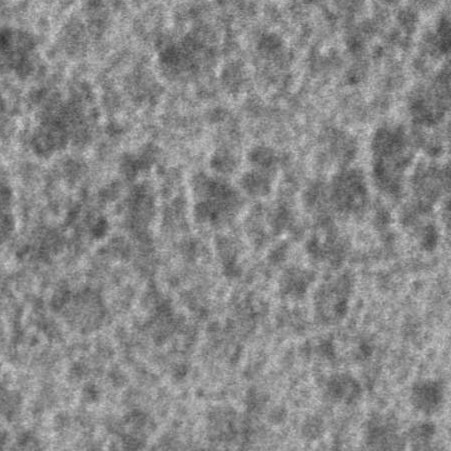
\includegraphics[width=250pt,center]{Image6_451_451.jpg}
		\caption{Вырезанное из снимка 6 изображние 451 на 451 пикселей}
	\end{figure}

	\subsection*{Результаты}
	\addcontentsline{toc}{subsection}{Результаты}
	\large
	\begin{figure}[h]
		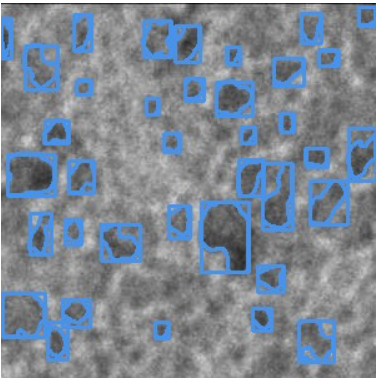
\includegraphics[width=250pt,center]{Image6_300_300_result.png}
		\caption{Результат вырезанного из снимка 6 изображeние 300 на 300 пикселей}
	\end{figure}
	\begin{figure}
		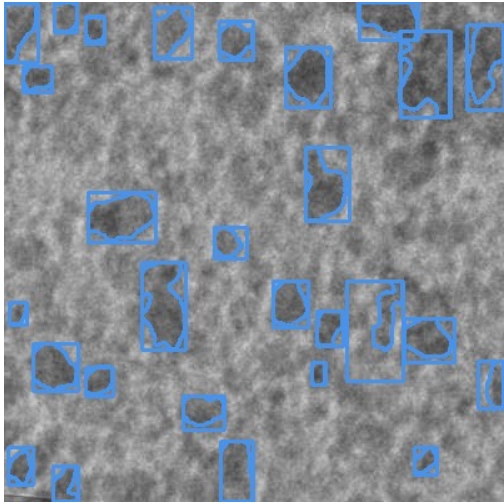
\includegraphics[width=250pt,center]{Image6_400_400_result.png}
		\caption{Результат вырезанного из снимка 6 изображeние 400 на 400 пикселей}
	\end{figure}
	\begin{figure}
		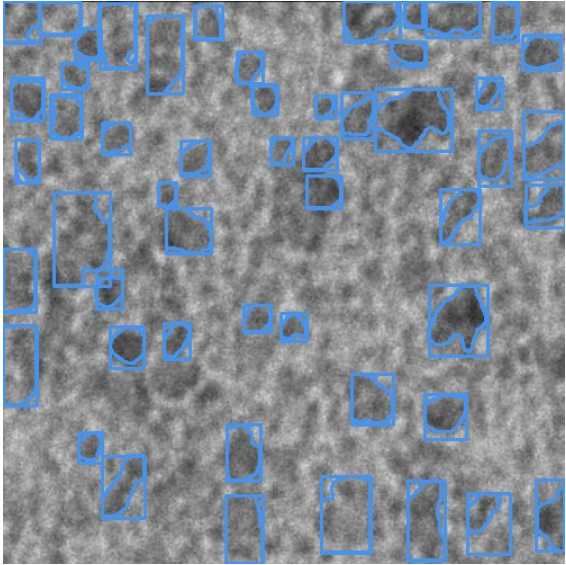
\includegraphics[width=250pt,center]{Image6_500_500_result.png}
		\caption{Результат вырезанного из снимка 6 изображние 500 на 500 пикселей}
	\end{figure}
	\begin{figure}
		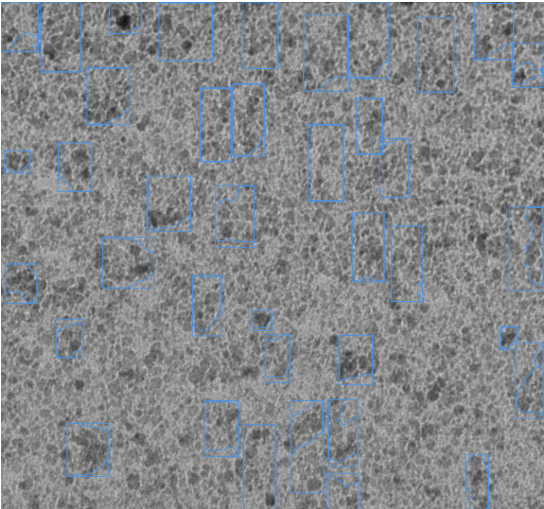
\includegraphics[width=250pt,center]{Image6_result.png}
		\caption{Результат снимка 6}
	\end{figure}

\end{document}
